\chapter{Background}
\label{ch:background}

\section{MathLang for Mathematics}
\label{sec:mathlang}

\begin{enumerate}
\item \textit{MathLang is} \textbf{a framework.} It is meant to be used for communication as a concrete support for human mind formulation. MathLang is a well structured framework aimed to synthesize the common mathematical language.

\item \textit{MathLang is} \textbf{for mathematics}. It is meant to be open to any branch of mathematics and to any topic that uses mathematics as a base language. MathLang mimics mathematics in its incremental construction of a body of knowledge.

\item \textit{MathLang is} \textbf{for computerisation.} MathLang is meant to be a medium for a human-system, human-human via a digital support, and system-system communication. MathLang is a computer-based framework and therefore offers automation facilities.

Taken from Maarek's thesis \cite{manuelphd}.

MathLang's original Goals, when the project started in 2000 was to allow a gradual computerisation and formalisation of mathematical texts.

\end{enumerate}

MathLang is not a system for proof verification but a framework to computerise and translate information (such as mathematical text) into a form on which proof checkers can operate.

The MathLang framework provides extra features supporting more rigour to translation of the common mathematical language. One can define further levels of translations into more semantically and logically complete versions. This gradual computerisation method should be more accessible than direct formalisation, because a number of first levels do nor require any particular expertise in formalisation.

So far Mathlang has given alternative and complete paths which transform mathematical texts into new computerised and formalised versions. Dividing the formalisation of mathematical texts into a number of different stages was first proposed by N.G. de Bruijn to relate common mathematical language to his Mathematical Vernacular \cite{mv} and his proof checking system Automath.

\subsection{The Current MathLang Design \label{sec:currentmath}}
The MathLang Framework instructs the computerisation process to be broken up into a number of levels called \textbf{aspects}. Having an aspect prevents the misunderstanding of the process of computerisation of mathematical documents using the MathLang Framework. Each aspect can be worked out independently, simultaneously or sequentially without prior knowledge of another aspect. The current MathLang Framework contains three well-developed aspects, the \gls{cga}, the \gls{tsa} and the \gls{dra}, and has further aspects such as the Formal Proof Sketch.

\begin{figure}[H]
\begin{center}
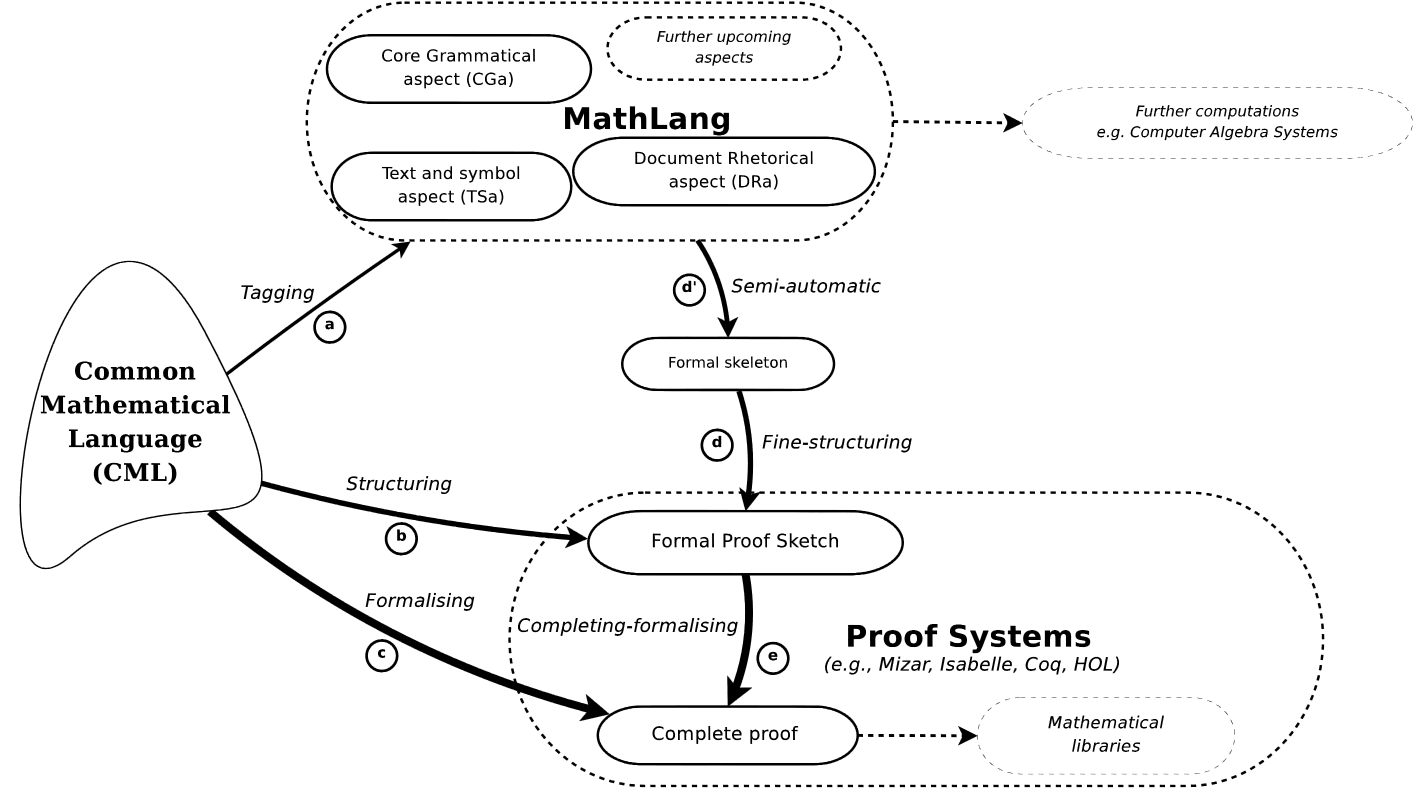
\includegraphics[scale=0.255]{Figures/Background/mathlang.png}
\end{center}
\caption{The MathLang approach to computerisation/formalisation \cite{mathintomizar}\label{fig:mathlang}}
\end{figure}

Figure \ref{fig:mathlang} shows the overall situation of work in the current MathLang Framework.
The labelled arrows show the computerisation paths from the common mathematical language to any proof system. The width of the arrow representing each path segment increases according to the expertise required to achieve the path segment. The level of expertise needed to computerise a CML text straight into a complete proof is very high, however the level of expertise is much smaller by using the MathLang framework to help form a formal skeleton and then into a complete proof. The dashed arrows illustrate further computerisation that one can envision.

\subsection{Core Grammatical aspect \label{subsec:cga}}
The current \gls{cga} in MathLang uses a finite set of grammatical \textit{categories} to identify the structure and common concepts used in mathematical texts. The aims of the \gls{cga} is to make explicit the grammatical role played by the elements of mathematical texts and to allow the validation of the grammatical and reasoning structure within the \gls{cga} encoding in a mathematical text. The \gls{cga} checks for grammatical correctness and finds errors like an identifier being used without and prior introduction or the wrong number of arguments being given to a function \cite{krzysztofphd}.

\subsection{Text and Symbol aspect \label{subsec:tsa}}
The \gls{tsa} builds the bridge between a mathematical text and its grammatical interpretation. The \gls{tsa} is a way of rewriting parts of the text so they have the same meaning. For example some mathematicians may prefer to write "a=b and b=c and c=d", others may prefer "a=b, b=c, c=d" and some others may prefer "a=b=c=d". As you can see all these methods of writing have the same meaning however some symbols are different. The \gls{tsa} annotates each expression in the text with a string of words or symbols which aim to act as the mathematical representation of which this expression is. This allows everything in the text to be uniform.

\subsection{Document Rhetorical aspect \label{subsec:dra}}

The Document Rhetorical aspects checks that the correctness of the reasoning in the mathematical document is correct and that there are no loops.The \gls{dra} mark-up system is simple and more concentrated on the narrative structure of the mathematical documents whereas other previous systems (such as DocBook \footnote{http://www.docbook.org}, Text Encoding Initiative \footnote{http://www.tei-c.org/index.xml}, OMDoc \footnote{http://www.omdoc.org}) were more concentrated on  the subtleties of the documents. It is used to describe and annotate chunks of texts according to their narrative role played within the document \cite{krzysztofphd}. Using the \gls{dra} annotation system we can capture the role that a chunk of text imposes on the rest of the document or on another chunk of text. This leads to generating dependency graphs which play an important role on mathematical knowledge representation. With these graphs, the reader can easily find their own way while reading the original text without the need to understand all of its subtleties. Processing \gls{dra} annotations can flag problems such as cicular reasoning and poorly-supported theorems.

\subsection{Full formalisation paths into Theorem Provers}

The MathLang project starts in 2000 when F.Kamareddine and J.B. Wells started the project within Heriot-Watt University as part of the ULTRA group \cite{researchprop}. It was an idea for a new mathematical language and framework to keep most of the advantages of Common Mathematical Language (CML) and avoid it's disadvantages. This framework would allow a gradual computerisation and formalisation of mathematical texts.

The framework was first set out in 2003 \cite{firstyear} and then saw an established path for conversion of a mathematical text written in CML into the isabelle proof assistant using rules and MathLang annotations \cite{secondyear}. A few short projects (by 4th year undergraduate dissertations or MSc students) have developed MathLang into the Framework it is today. A prototype of the Core Grammatical aspect and Text and Symbol aspect were defined in the PhD thesis of Manuel Maarek \cite{manuelphd} and then a gradual computerisation into the Mizar proof assistant using the three key aspects of MathLang were a great success and published \cite{mathintomizar}.

The design of the \gls{cga} is due to Kamareddine, Maarek and Wells \cite{oomathlang} and the implementation of the \gls{cga} is due to Maarek \cite{manuelphd}. The design of the \gls{tsa} is due to Kamareddine, Maarek, and Wells with contributions by Lamar to the souring rules \cite{restoringtsa}, \cite{manuelphd}, and \cite{lamarphd}. The implementation is primarily by Maarek \cite{manuelphd} with contributions from Lamar \cite{lamarphd}. The design and implementation of \gls{dra} were the subject of Retel's thesis \cite{krzysztofphd}. Further additions have since been carried out by Zengler \cite{cmtim}.

\subsection{Conclusion}
A lot of work has already been completed on the MathLang Framework. The three aspects, \gls{cga}, \gls{dra}, and \gls{tsa}, have been designed and redesigned so that a variety of mathematical texts and symbols could be used. Then the aspects have been implemented for ease of access. A translation from a mathematical text into the Mizar proof checker has been worked through and described in detail in a published paper \cite{mathintomizar} and a PhD thesis \cite{manuelphd}. A partial translation from a CML text into the Isabelle Syntax has also been carefully described in the 2009 paper \cite{mathintoisa} and also written in a PhD thesis \cite{lamarphd}. Some of the future work described was to allow MathLang to be used as a tool to computerise other pieces of information, such as another piece of academic text yet it does not need to be mathematical.

\section{Formal Notation}
\label{sec:formnot}

\subsection{Tools for Z}
\label{subsec:tools}